\documentclass{standalone}
\begin{document}
	\subsection*{Training}
	
	This step involves the estimation of the centroid set. To achieve this purpose, k-means clustering was performed on a training set made on multichannel images from many CT scans. During this task, I have to take into account that k-means clustering requires a balance in the different cluster representation. As we can see in \figurename\,\ref{fig:ClusterRepr}, the main part of the image is composed of background, that is an over-represented cluster. Moreover, we can observe that the amount of involved lung volume may change according to the severity of the disease: the first scan presents a low amount of GGO and CS; the second one has a larger lung region involved.

	\begin{figure}[h!]
		\centering
		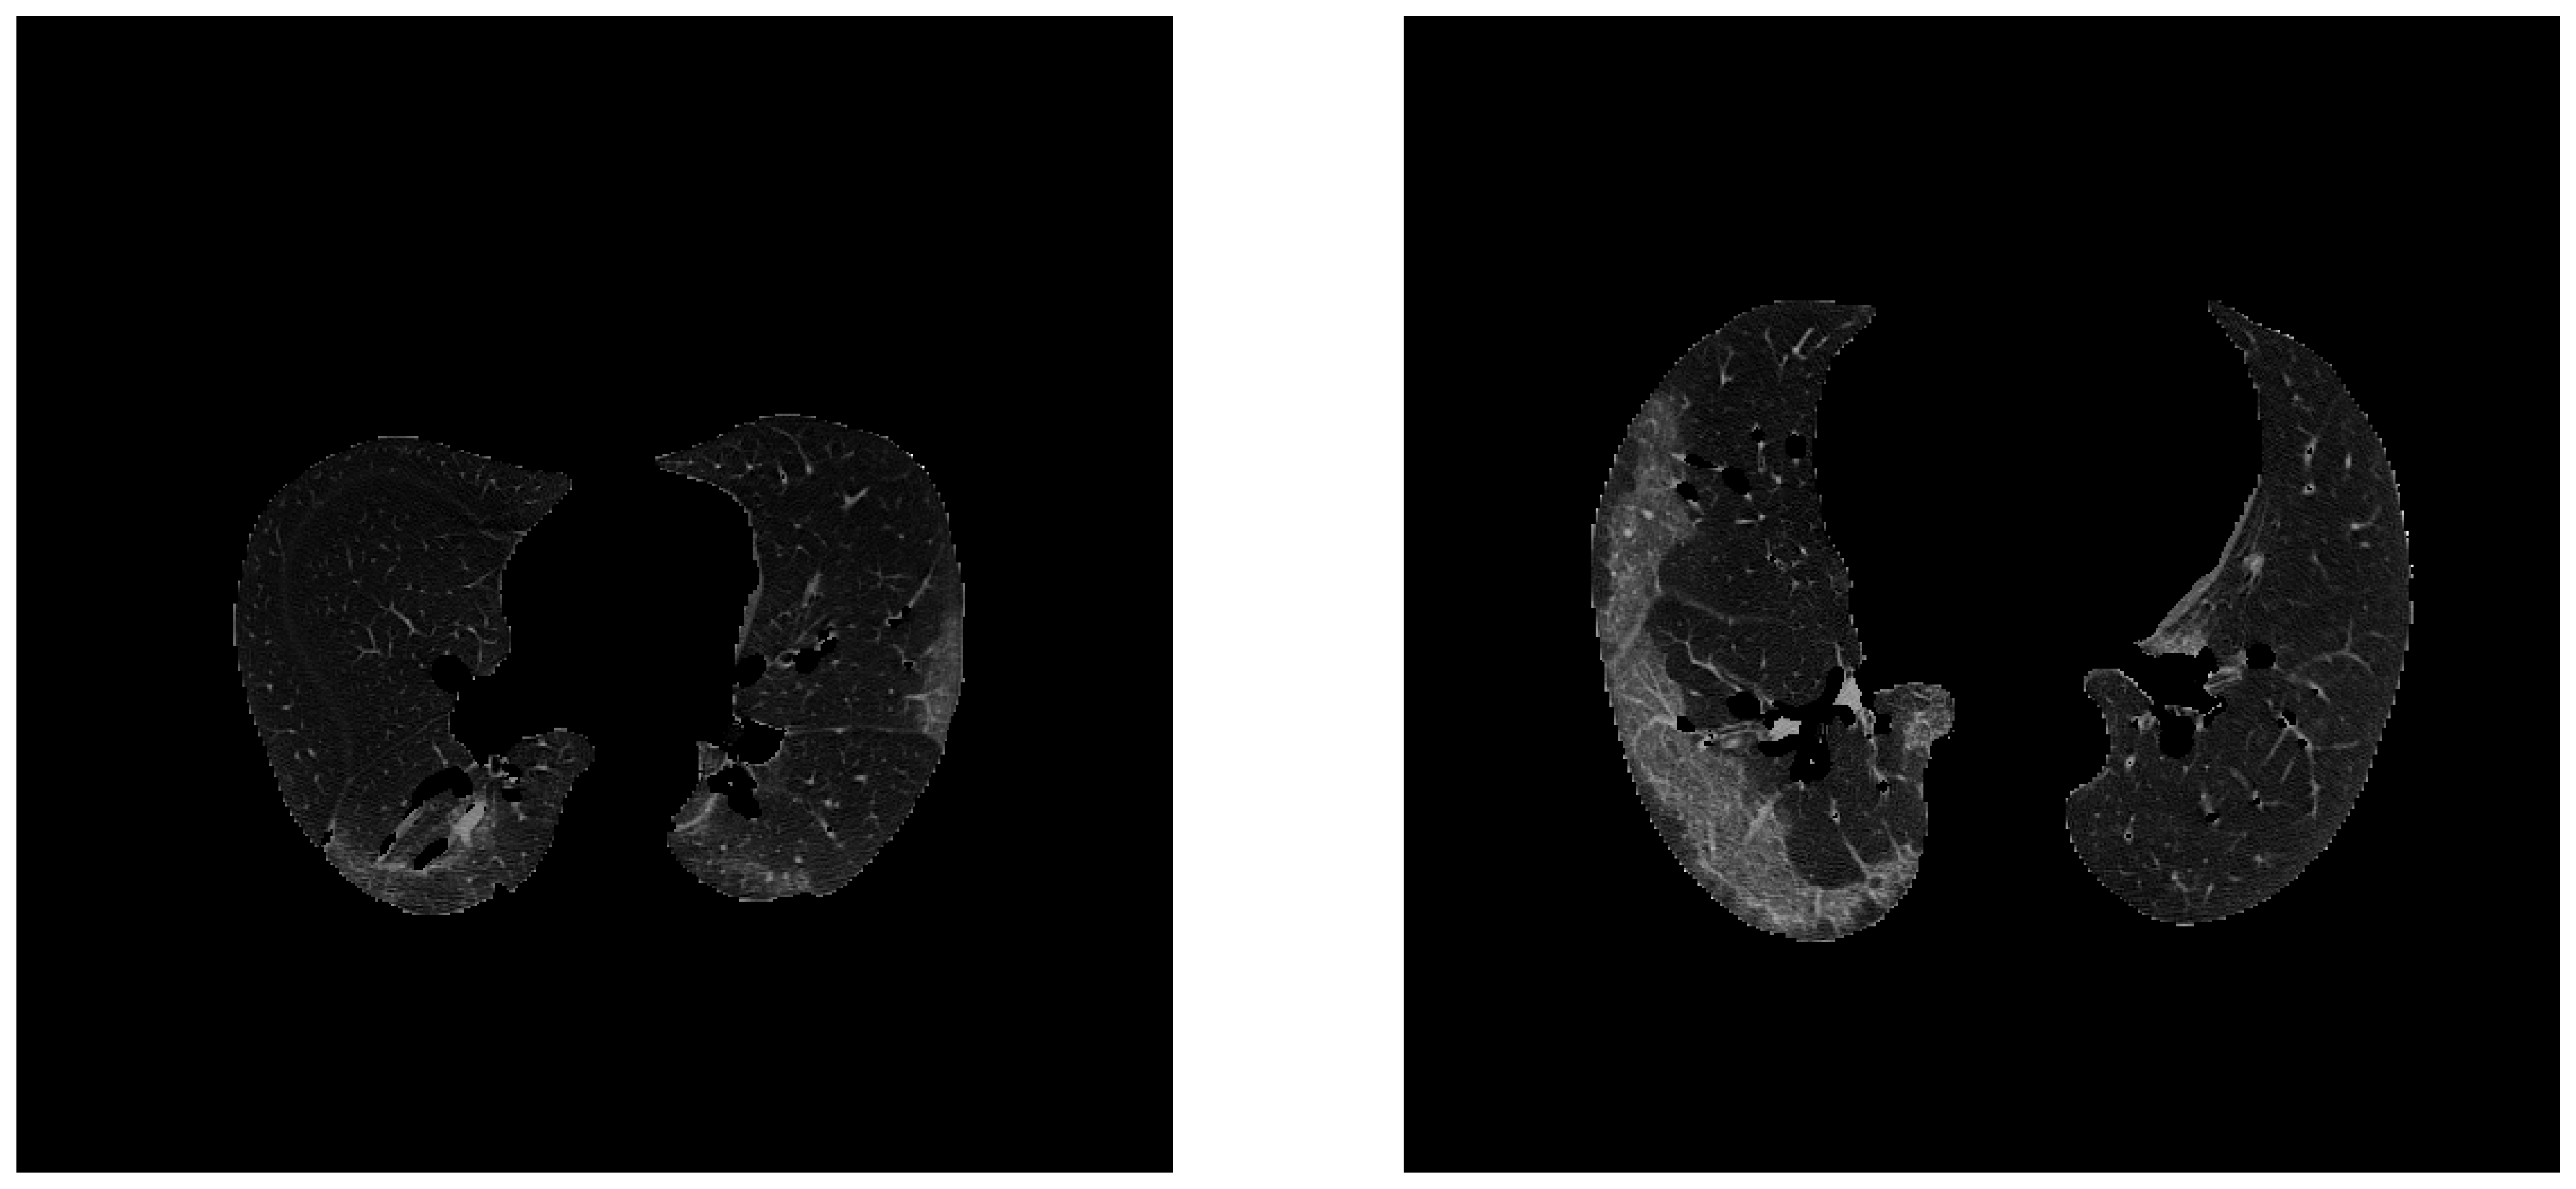
\includegraphics[scale=.4]{ClusterRepr.png}
		\caption{Lung regions with different ground-glass areas. We can notice that the main part of the image is composed only by the background. From left to right respectively a scan with small lesion areas and one with a large lesion.}\label{fig:ClusterRepr}
	\end{figure}

	
	The images of the training set are then shuffled and split into many subsamples and the clustering is performed independently on each one of them. As a final centroid set, I have considered the one that minimizes the intra-cluster variance. This step is justified since the results of the k-means clustering depend on the initial choice centroids. During the minimization of the potential function, the algorithm may find a local minimum rather than the global one. The different clustering allows to estimate more than one possible solution and to choose the best one. Moreover, the creation of several sub-samples is made since the creation of a single, large array with several images is not always possible, since requires a huge quantity of memory to be allocated.
\end{document}	
